\chapter{Дартс}

Този проект представлява популярната дартс игра. Играчът хвърля къси стрели по кръгла мишена. Колкото по- близо е до центъра на мишената, толкова повече точки печели. Целта на играча е да събере максимален брой точки за трите удъра, с които разполага. Ако събраните точки са над 13 - печели играта, в противен случай губи играта.

\begin{figure}[H]
  \centering
  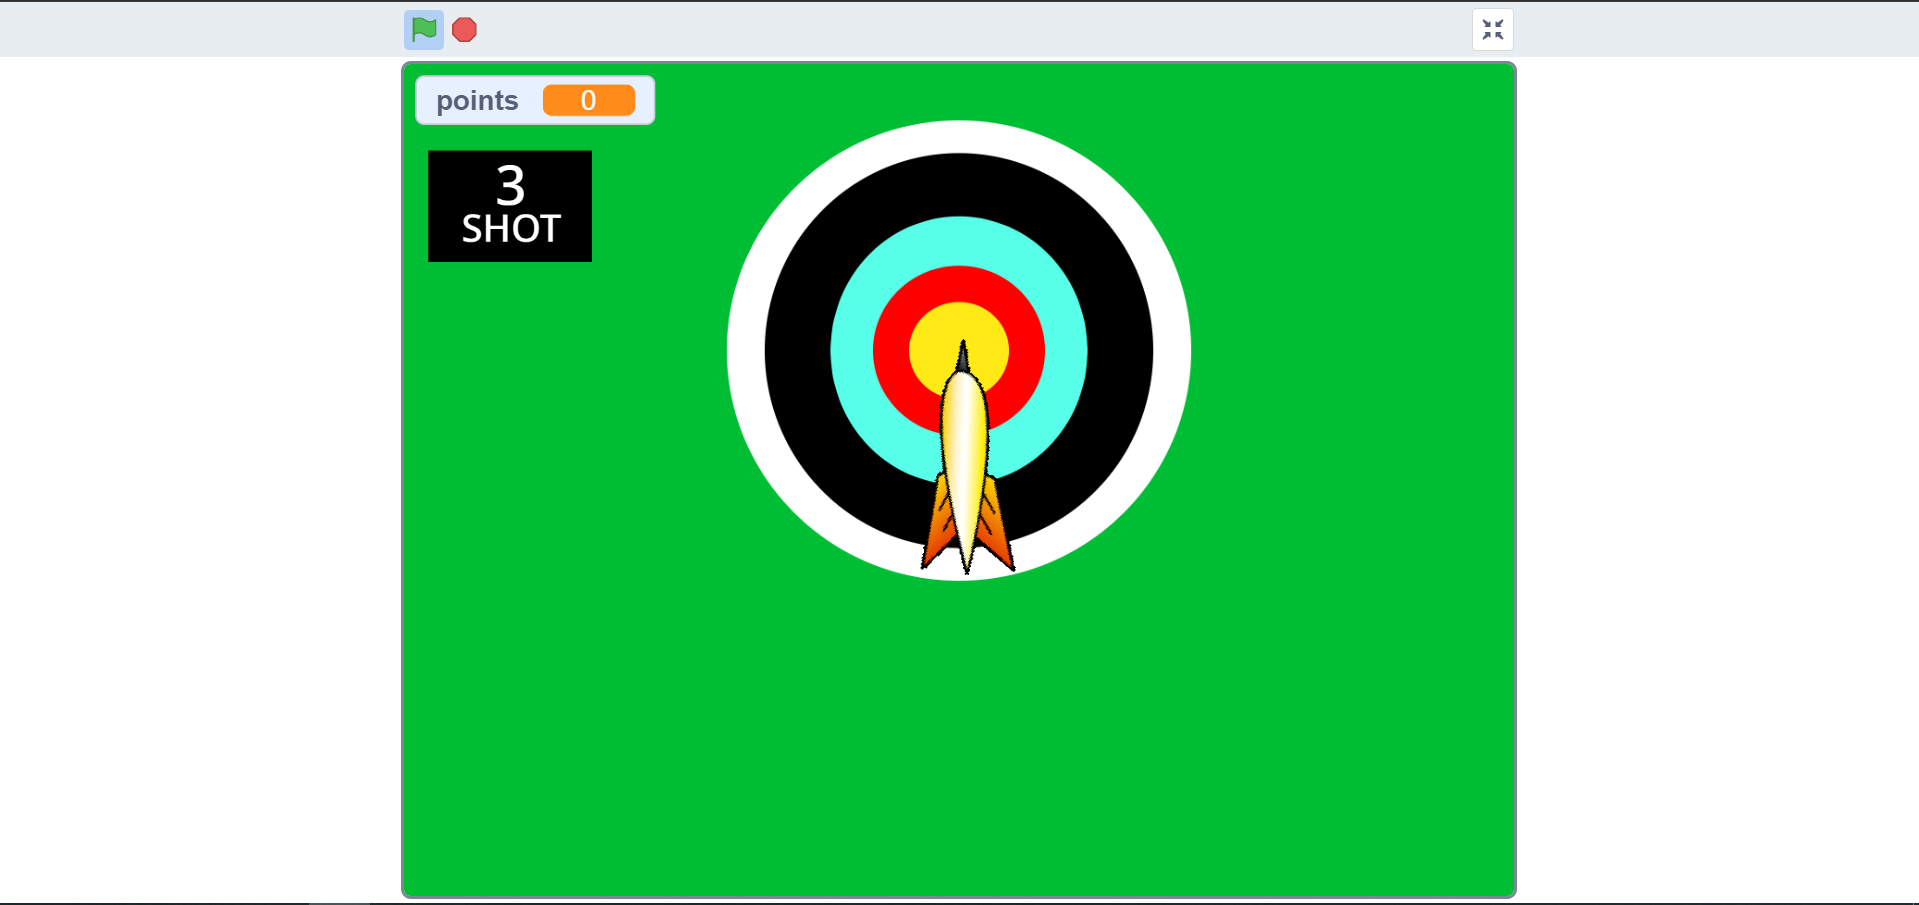
\includegraphics[width=1.0\linewidth,height=0.5\linewidth]{fig150001.png}
  \caption{Дартс}
\label{fig150001}
\end{figure}

\section{Създаване на дизайна}
Преди да започнете с програмирането на играта, първо трябва да създадете дизайна. Първо добавете двата основни героя на играта - мишената (Фиг. \ref{fig150002}) и стрелата (Фиг. \ref{fig150003}). Използвайте инструментите в Scratch, за да нарисувате необходимите герои.

\begin{figure}[H]
  \centering
  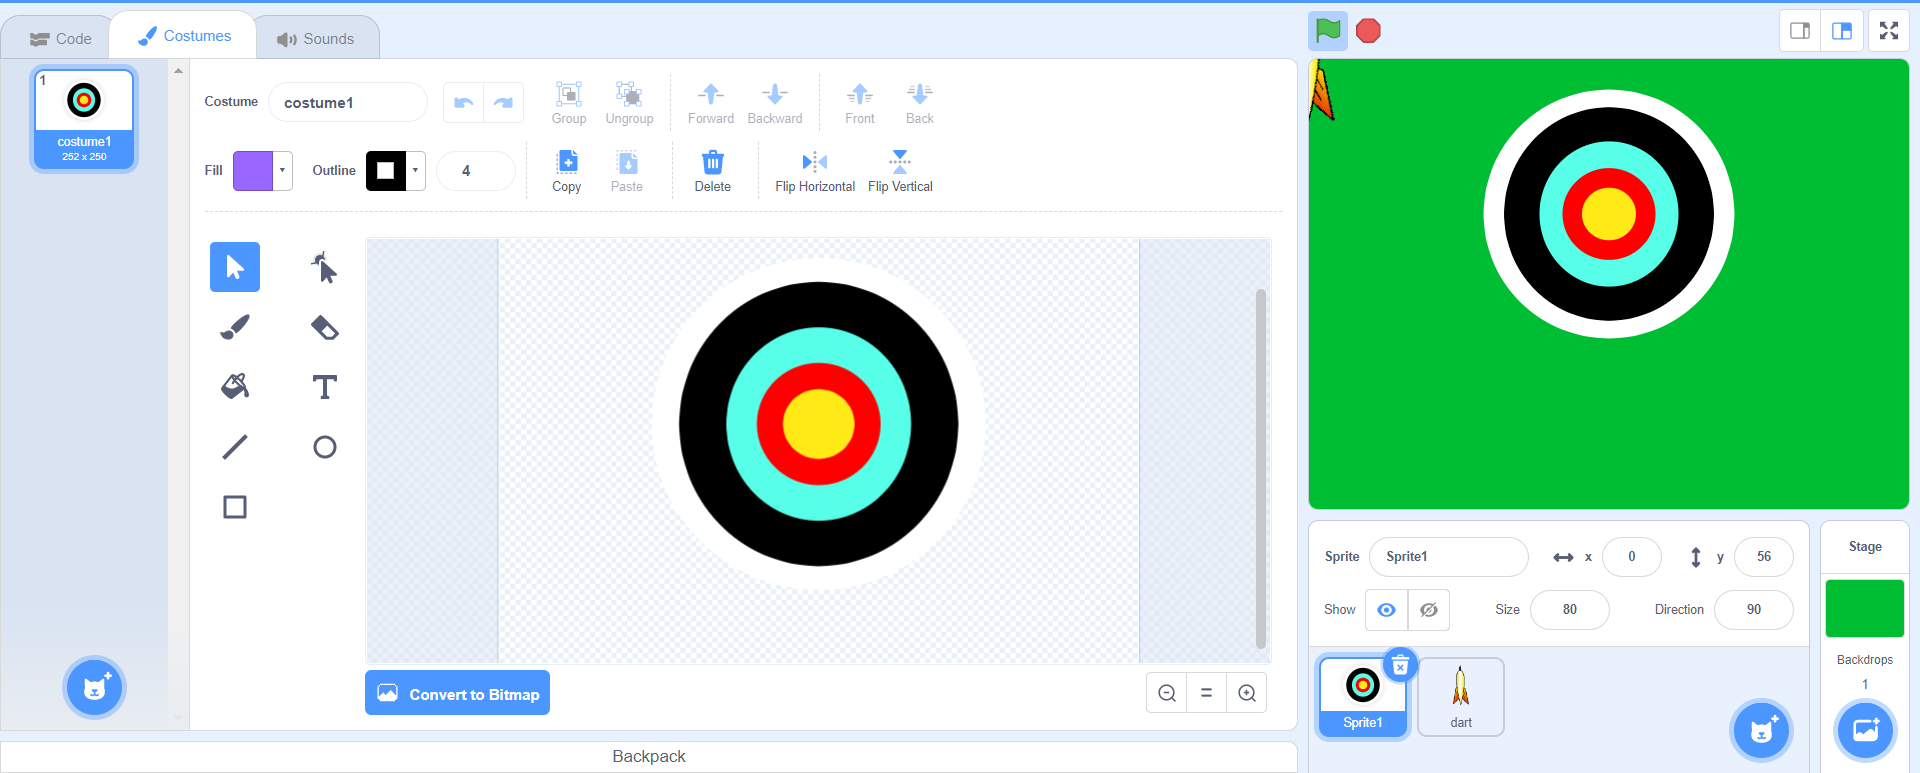
\includegraphics[width=1.0\linewidth,height=0.5\linewidth]{fig150002.png}
  \caption{Мишена}
\label{fig150002}
\end{figure}

\begin{figure}[H]
  \centering
  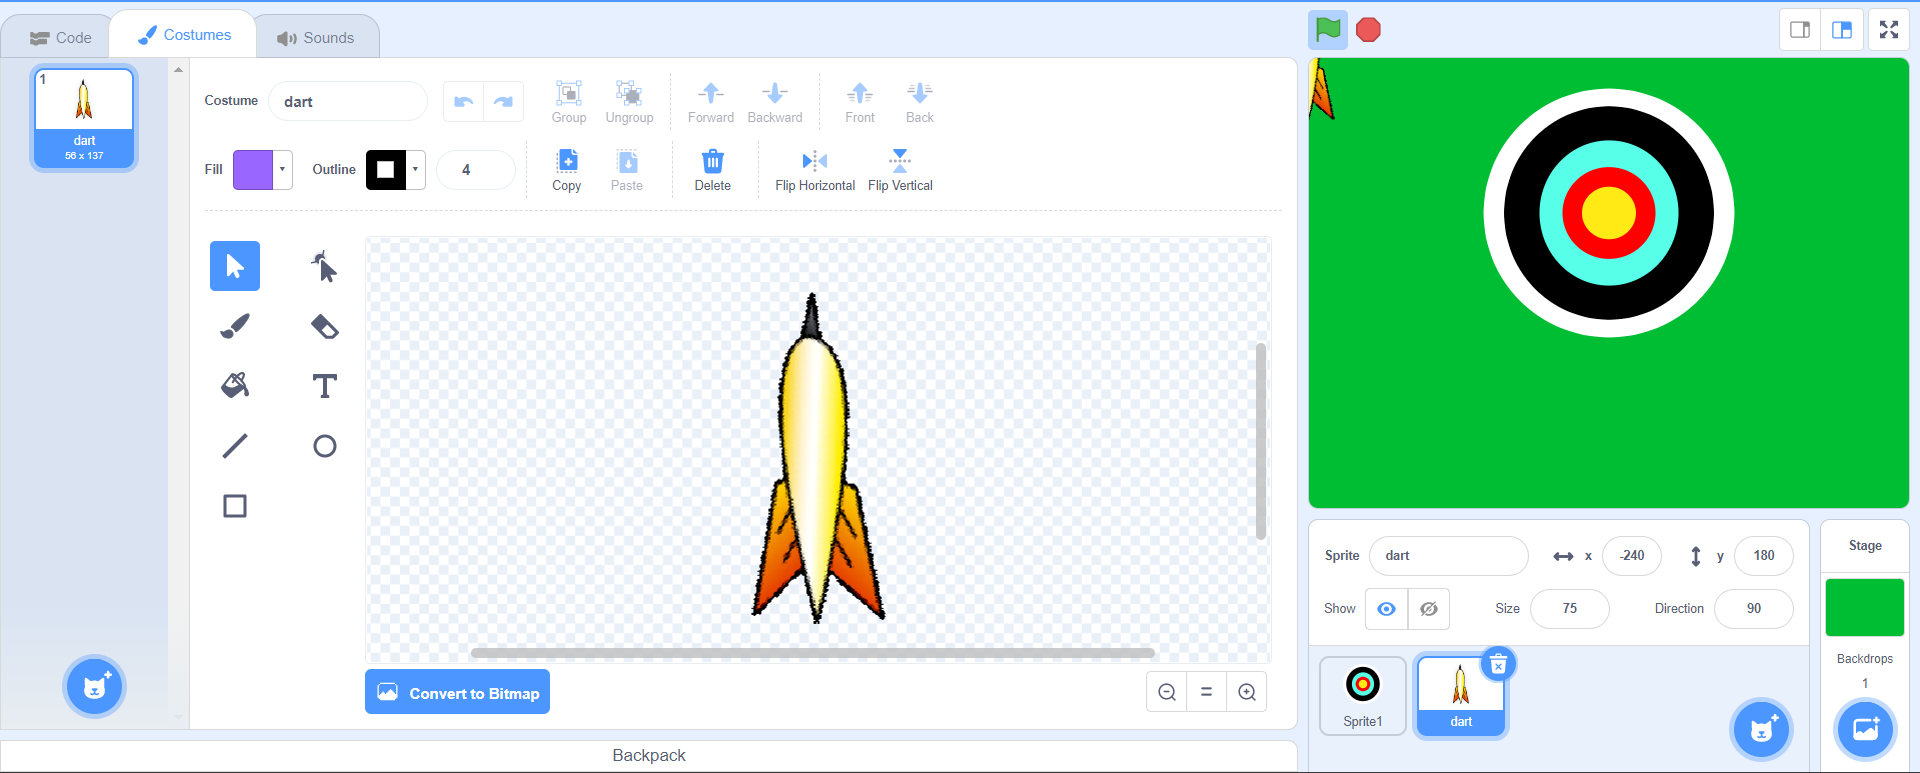
\includegraphics[width=1.0\linewidth,height=0.5\linewidth]{fig150003.png}
  \caption{Стрела}
\label{fig150003}
\end{figure}

Добавете нов герой, който също може да нарисувате с помощта на Scratch инструментите. Този герой ще бъде отговрен за това да показва колко изстрела остават на играча. За да покажете колко изстрела остават, добаявте костюми на този герой. Например на първия костюм може да напишете, че остават 3 изстрела, а на втория - 2 изстрела.

\begin{figure}[H]
  \centering
  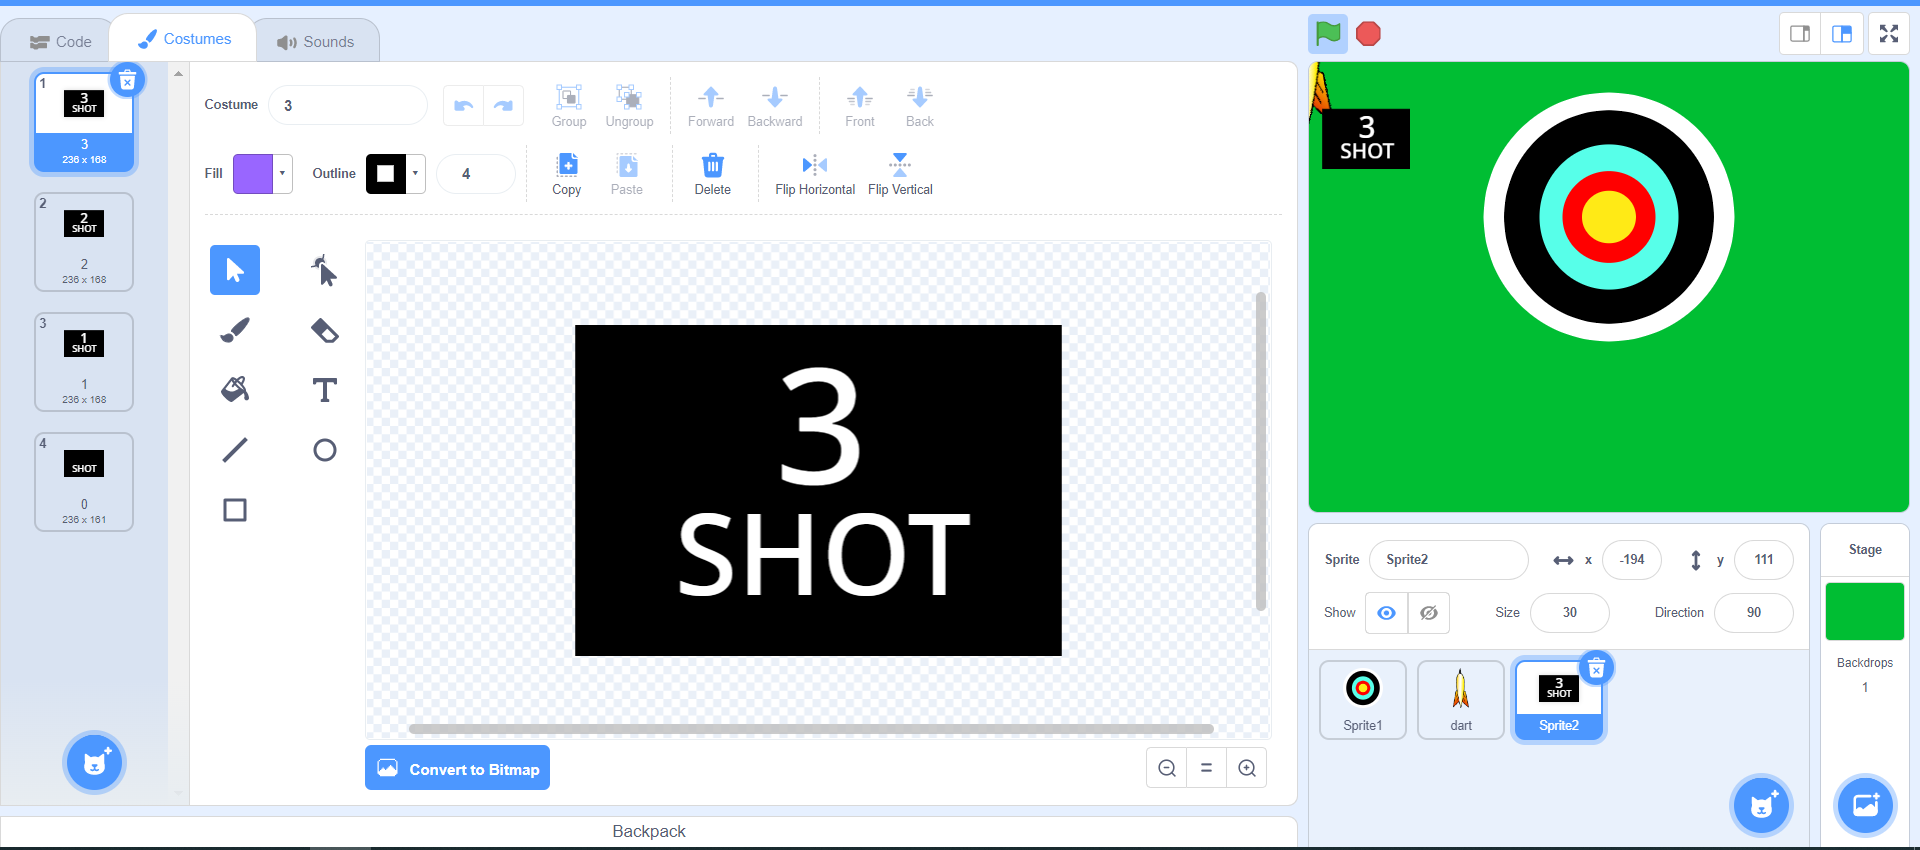
\includegraphics[width=1.0\linewidth,height=0.5\linewidth]{fig150004.png}
  \caption{Брой изстрели}
\label{fig150004}
\end{figure}

Следващият герой, който следва да добавите е, този, който показва колко точки е спечелил играчът. Отново добавете костюми на героя със съответния брой точки които той може да спечели. В случая това са от 0 до 5.

\begin{figure}[H]
  \centering
  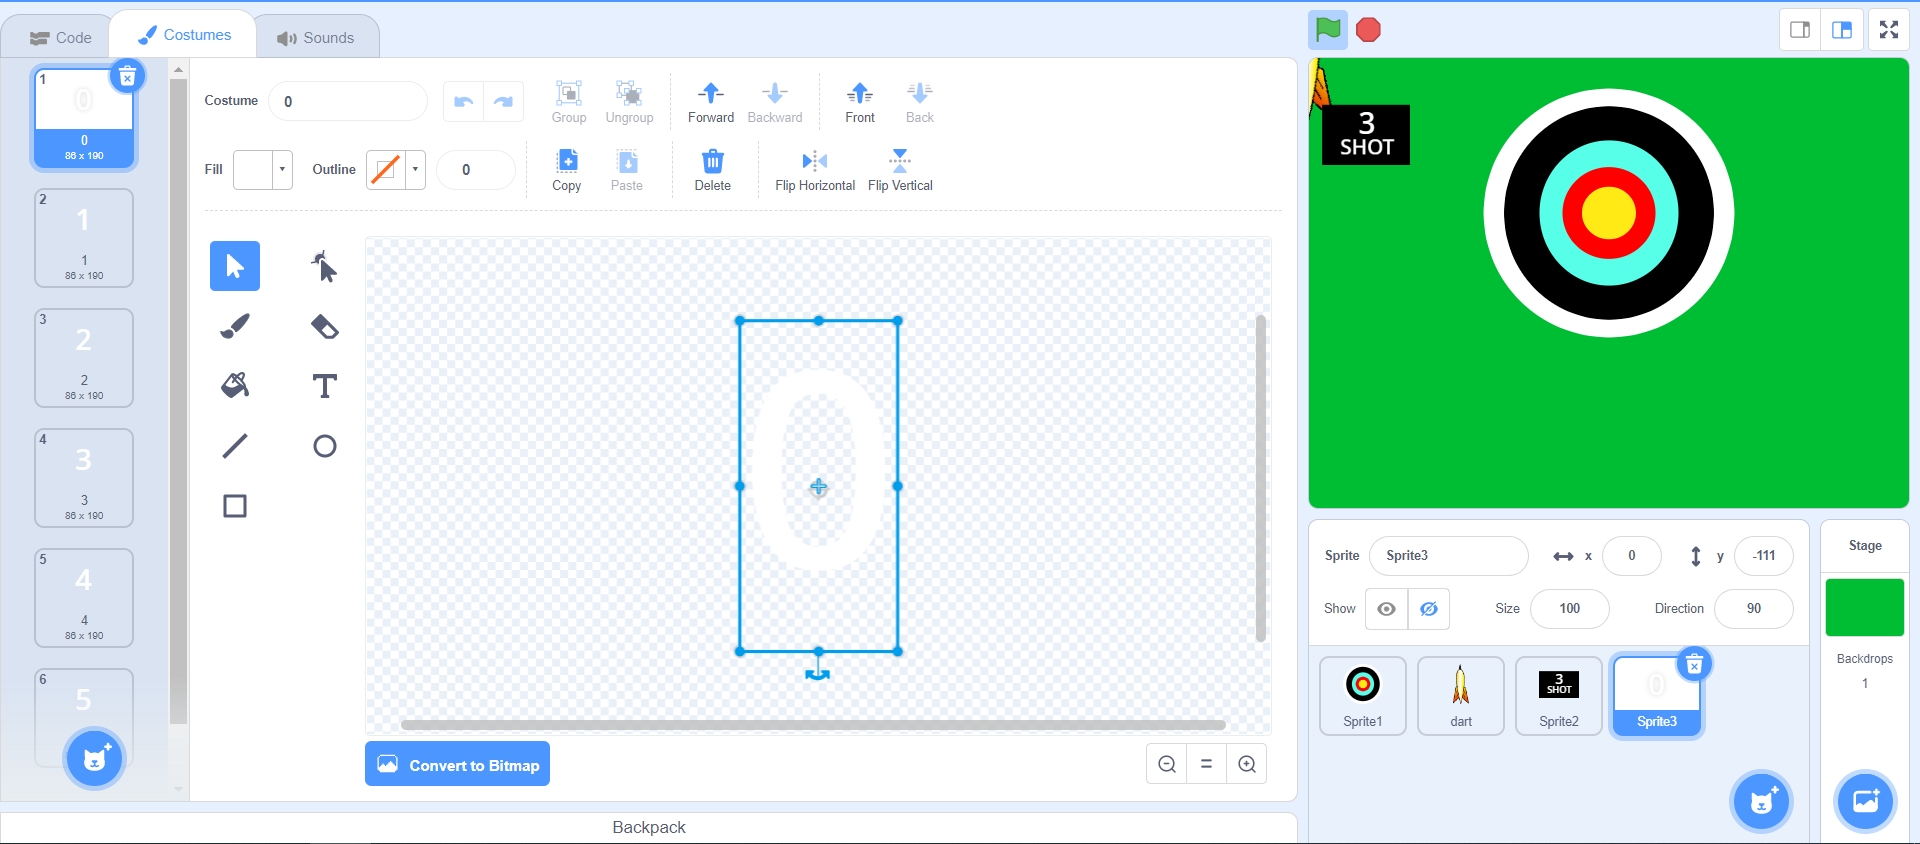
\includegraphics[width=1.0\linewidth,height=0.5\linewidth]{fig150005.png}
  \caption{Брой точки}
\label{fig150005}
\end{figure}

Последният Scratch герой е надписа дали играчът печели или губи. Подобно на предишните два героя, добавете два костюма с различни надписа - единият да бъде за победа, а другият за загуба.

\begin{figure}[H]
  \centering
  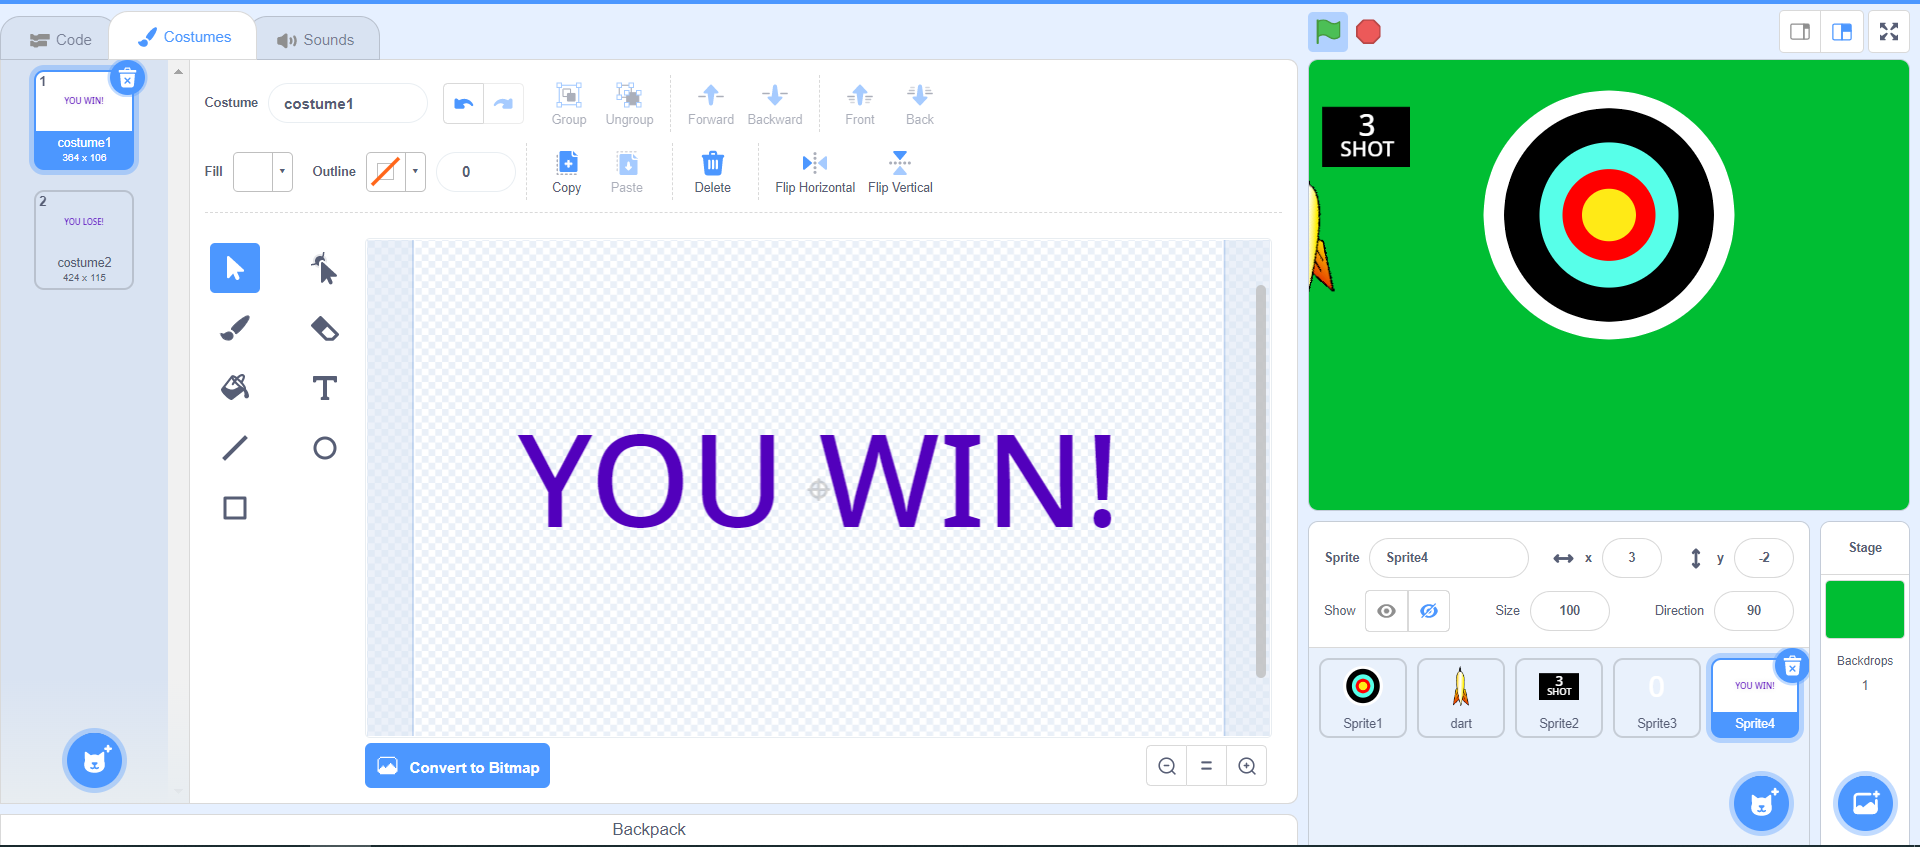
\includegraphics[width=1.0\linewidth,height=0.5\linewidth]{fig150006.png}
  \caption{Надпис за край на играта}
\label{fig150006}
\end{figure}

\section{Програмиране на мишената и стрелата}
Преди да преминем към порграмирането на съответните герои, добавете нова променлива points към играта. Тази променлива ще съдържа в себе си резултата, който героят ще трупа по време на играта. От секция Variables изберете Make a Variable и задайте име на променливата.

\begin{figure}[H]
  \centering
  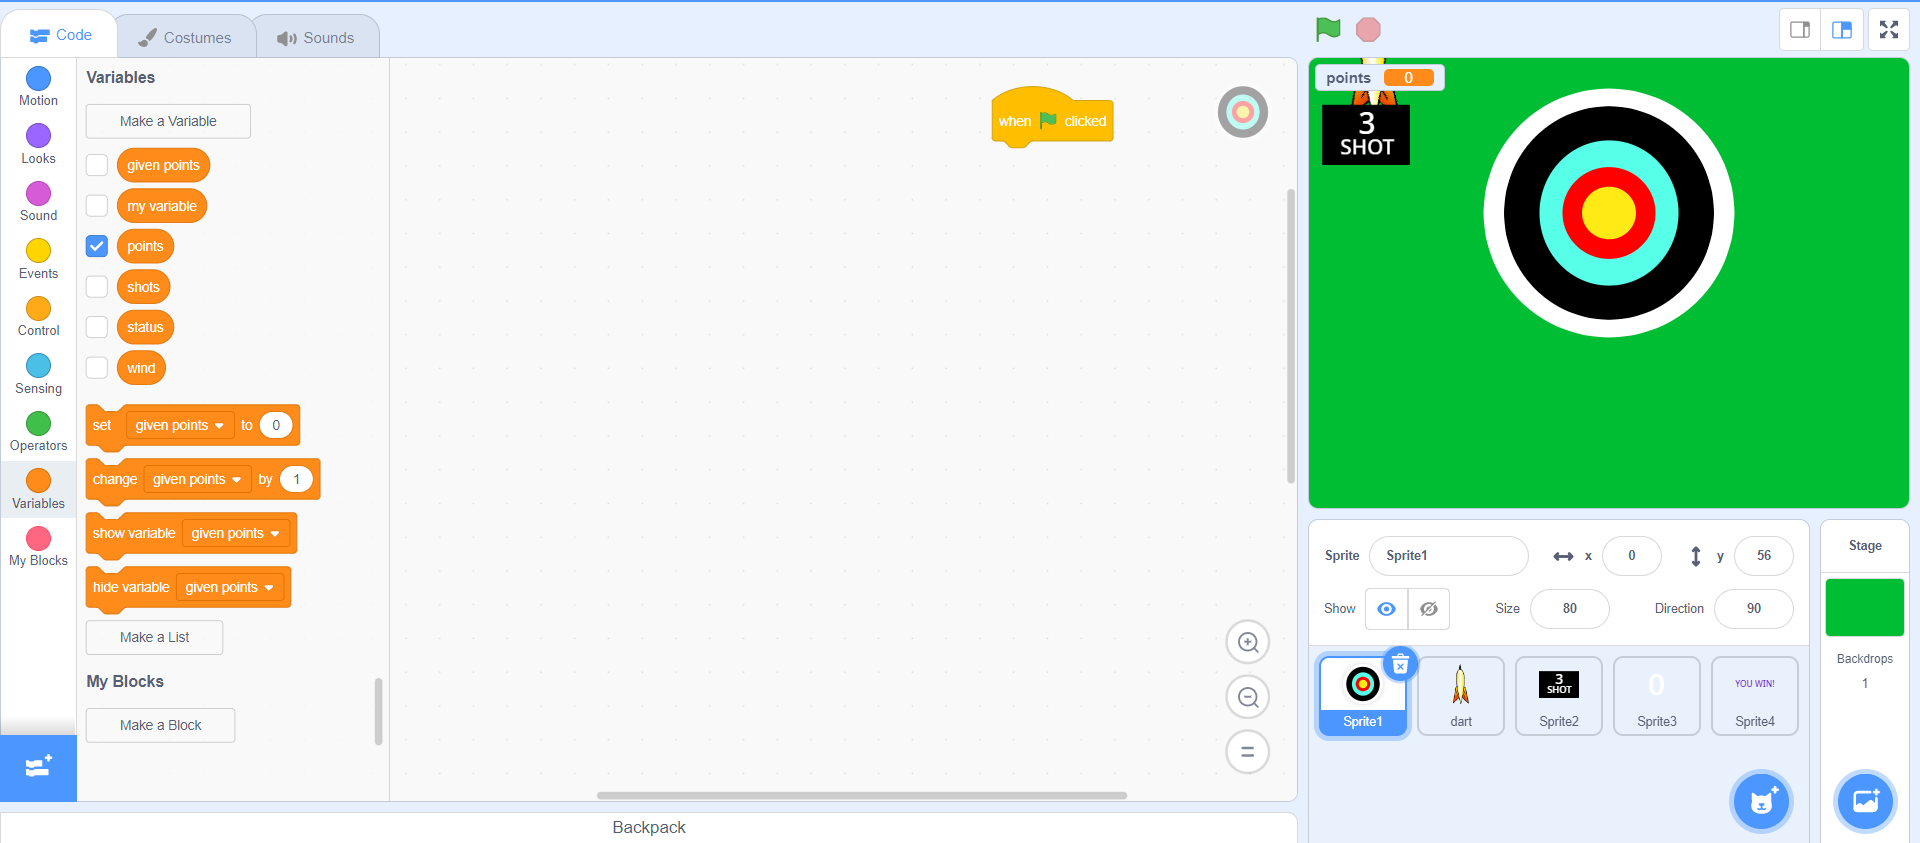
\includegraphics[width=1.0\linewidth,height=0.5\linewidth]{fig150007.png}
  \caption{Създаване на променлива в играта}
\label{fig150007}
\end{figure}

Нека да преминем към програмирането на мишената. Единствените инструкции, които трябва да добавите към този герой са, той да бъде на една и съща позиция по време на цялата игра. Не забравяйте да зададете и първоначална стойност на променливата, която създадохте. В началото на всяка игра, играчът трябва да има 0 точки.

\begin{figure}[H]
  \centering
  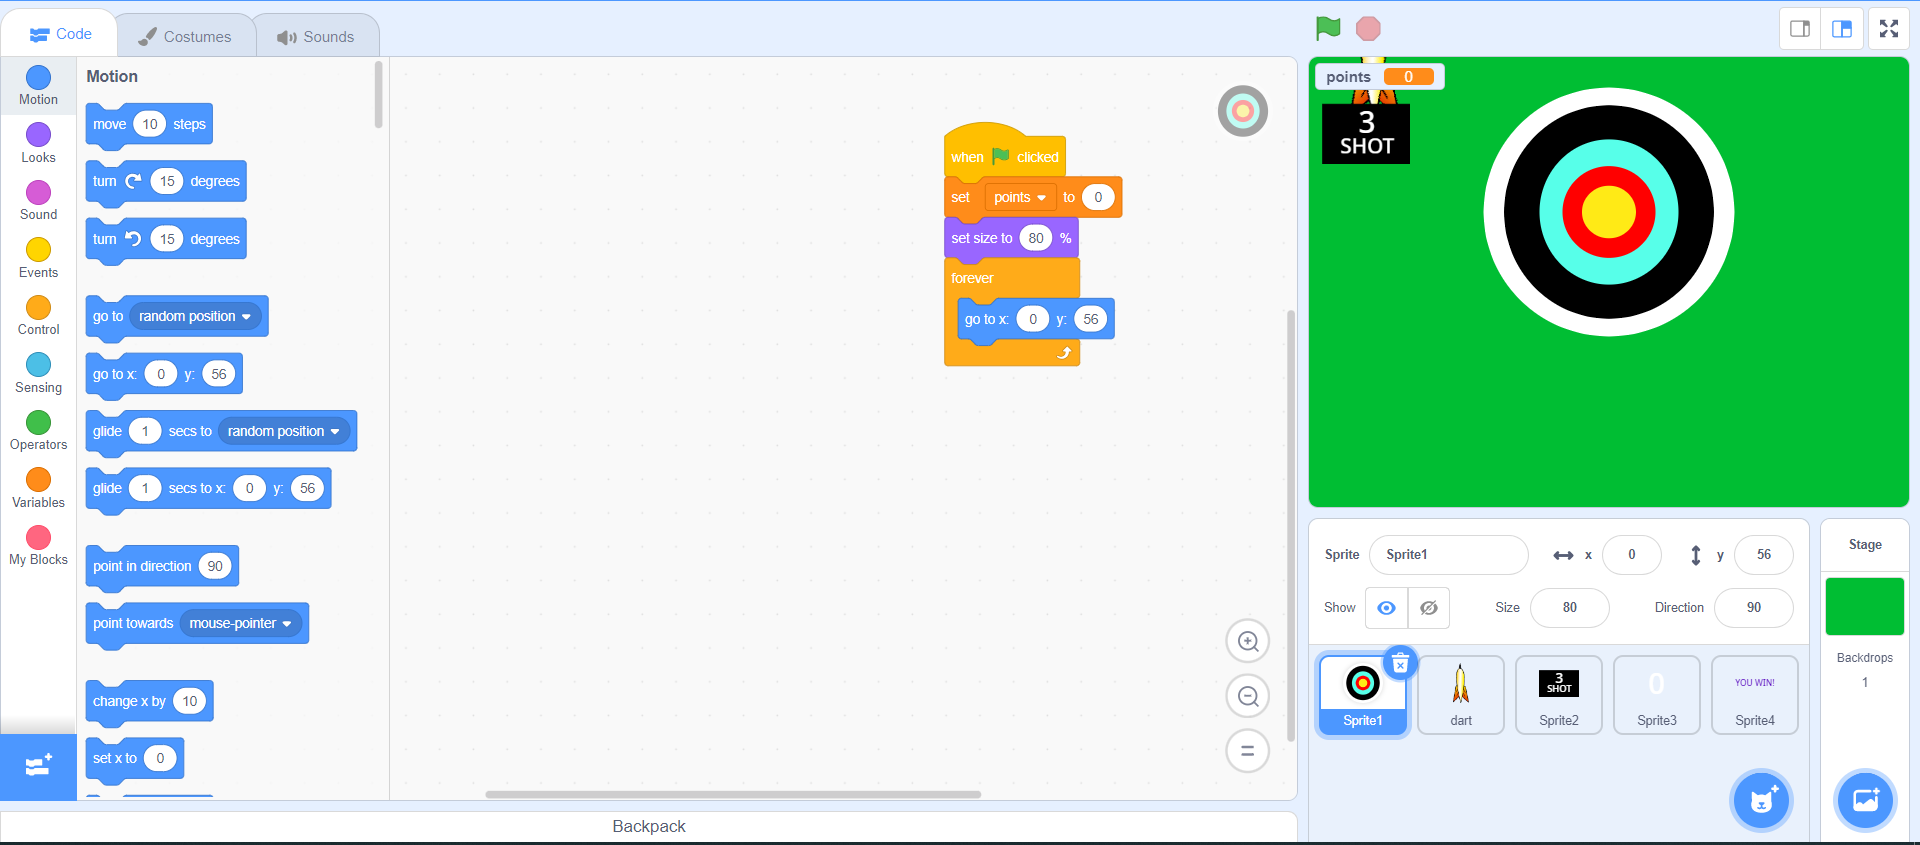
\includegraphics[width=1.0\linewidth,height=0.5\linewidth]{fig150008.png}
  \caption{Инструкции на мишената}
\label{fig150008}
\end{figure}

Следва да добавите инструкции и за стрелата. Ако стрелата в твърде голяма, може да промените размерите ѝ. Създайте нова променлива, която да съдържа в себе си какъв е статуса на стрелата. Съществуват два статуса - shoot или throw. В началото на играта статуса на стрелата ще бъде shoot.

\begin{figure}[H]
  \centering
  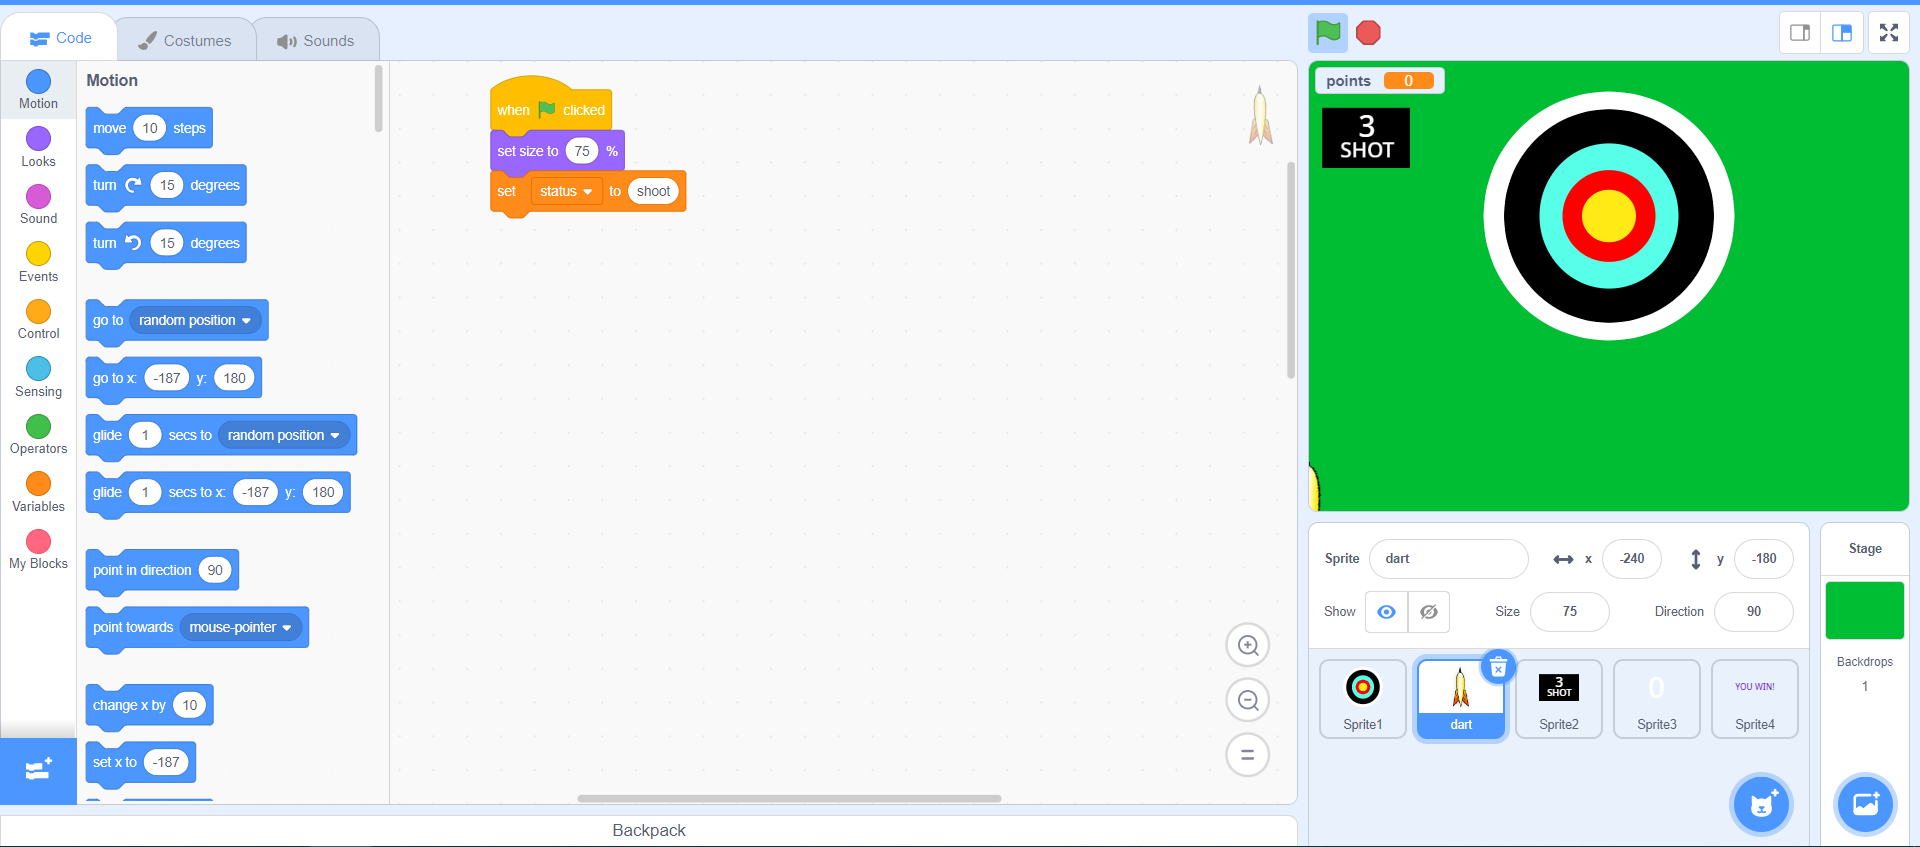
\includegraphics[width=1.0\linewidth,height=0.5\linewidth]{fig150009.png}
  \caption{Задаване на статус на стрелата}
\label{fig150009}
\end{figure}

Добавете следната проверка - ако статуса на стрелата е shoot, то тогава стрелата трябва да следва мишката на играча. Също така добавете и ново събитие, което е when this sprite clicked. Когато играчът кликне върху стрелата, трябва да промените стойността на променливата status да бъде throw. Също така героят трябва да изпрати съобщение на другите герои, че играчът е натиснал мишката, което означава, че стреля.

\begin{figure}[H]
  \centering
  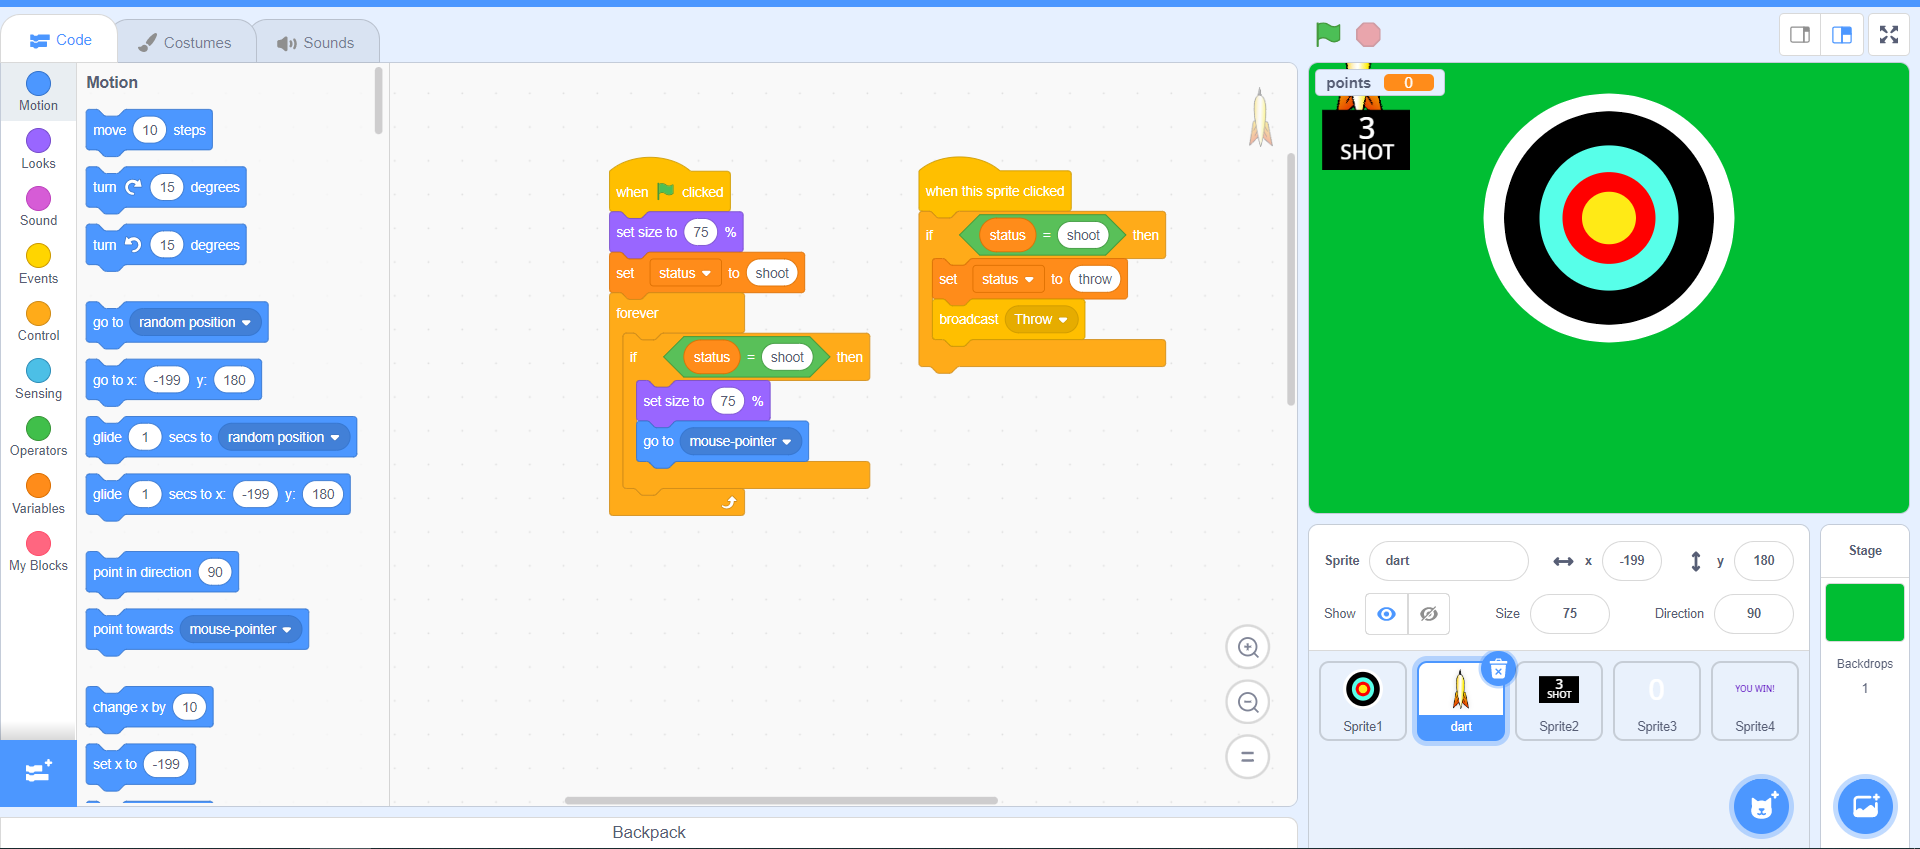
\includegraphics[width=1.0\linewidth,height=0.5\linewidth]{fig150010.png}
  \caption{Изпращане на съобщение за стрелба}
\label{fig150010}
\end{figure}

След като играчът е изстрелял стрелата трябва да я програмирате да променя посоката си, за да може да имитирате изстрел. Също така променете и размерите ѝ да става по- малка, все едно се отдаличава от играчът. Знаете, че когато играчът кликне върху стрелата, то се изпраща съобщение. Използвайте това съобщение за да промените посоката и размера на стрелата след изстрел.

\begin{figure}[H]
  \centering
  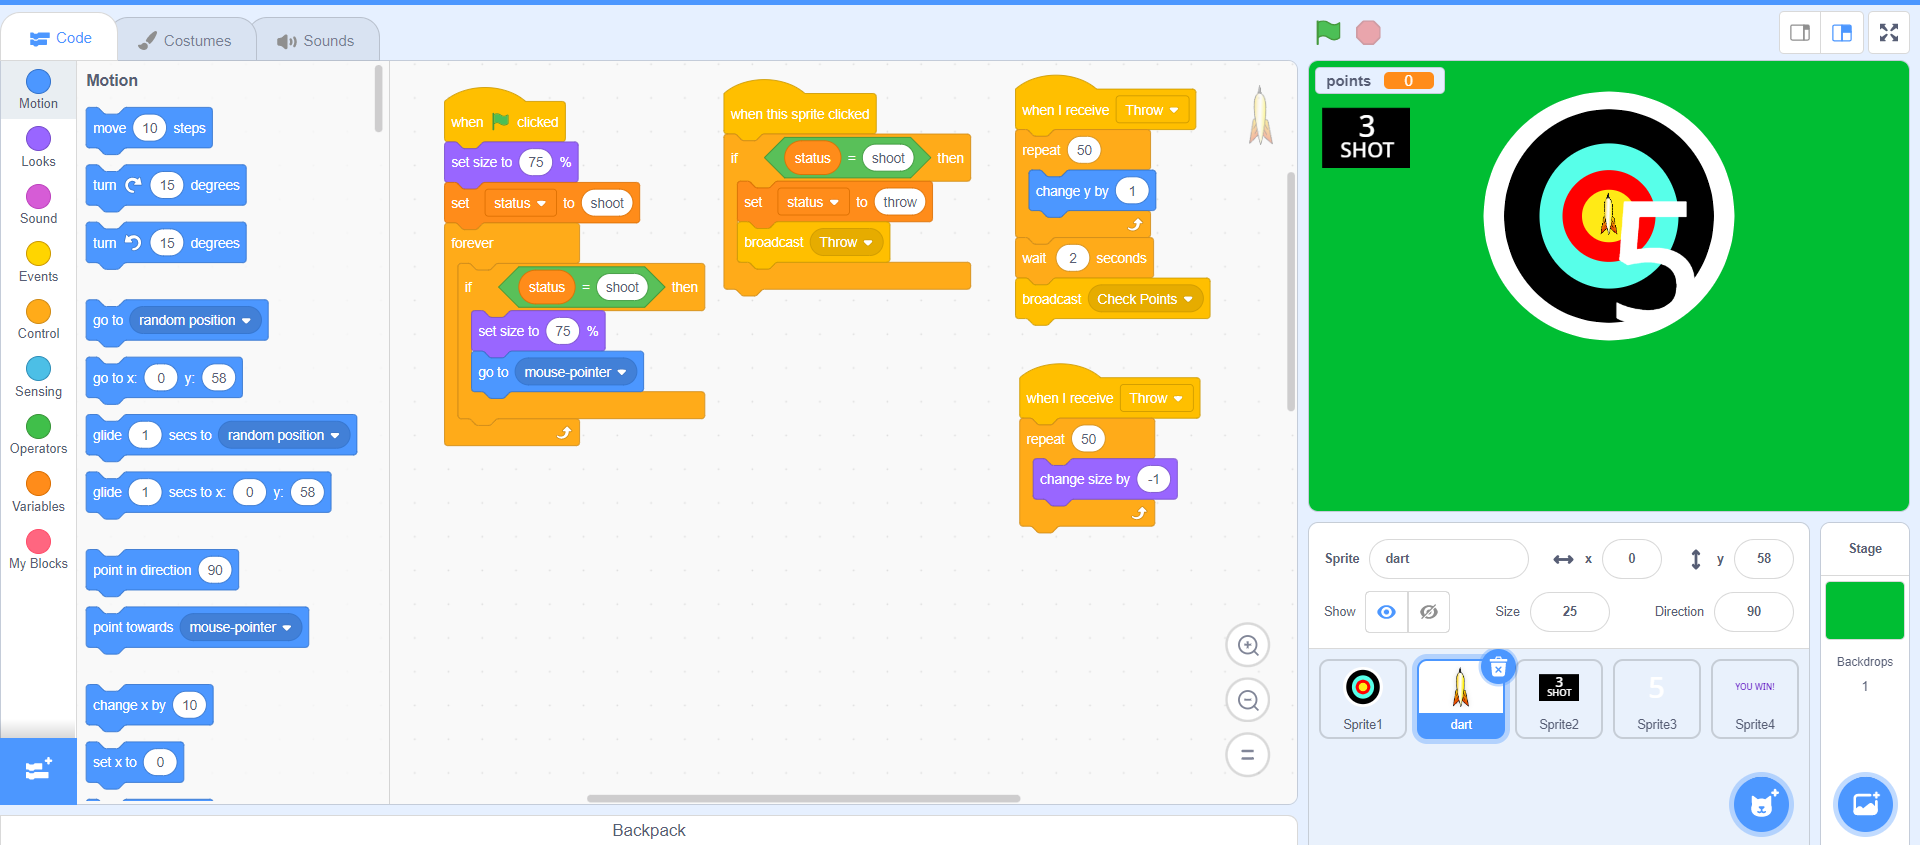
\includegraphics[width=1.0\linewidth,height=0.5\linewidth]{fig150011.png}
  \caption{Промяна на посоката и размера на стрелата след изстрел}
\label{fig150011}
\end{figure}

Когато играчът изстреля стрелата, тя започва да се отдаличава и изпраща съпбщение Check Points, което трябва да провери колко точки е спечелил играчът. За да се определи броя на спечелените точки, трябва да се провери до какъв цвят се е докоснала стрелата. За да бъде най- честна играта проверката, която ще се направи е черният цвят (това е върхът на стрелата) до кой цвят се е докоснал. Добавете нова променлива, която да съдържа текущо спечелните точки. Последната иснтрукция, която трябва да добавите е, стрелата да изпраща съобщение, че дава точки на играча.

\begin{figure}[H]
  \centering
  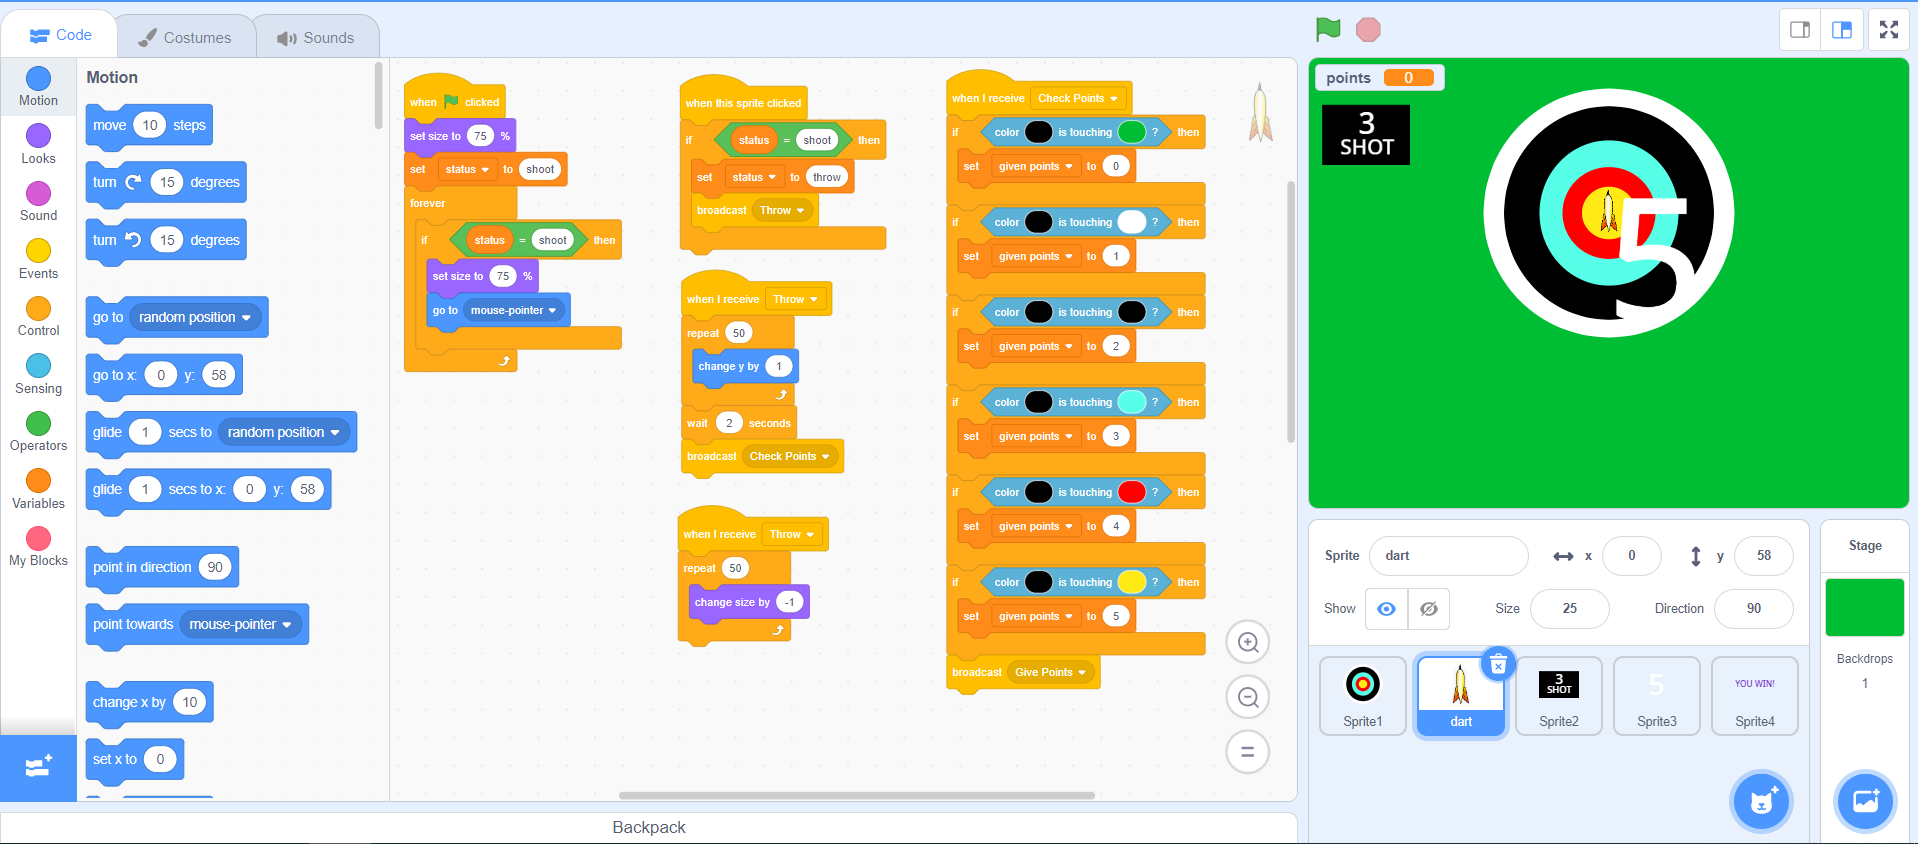
\includegraphics[width=1.0\linewidth,height=0.5\linewidth]{fig150012.png}
  \caption{Проверка на спечелените точки}
\label{fig150012}
\end{figure}

За да направите играта още по- интересна може да добавите променлива, която да бъде случайно зададено число. Тази променлива ще отклонява стрелата настрани, спрямо това какво случайно число се е паднало.

\begin{figure}[H]
  \centering
  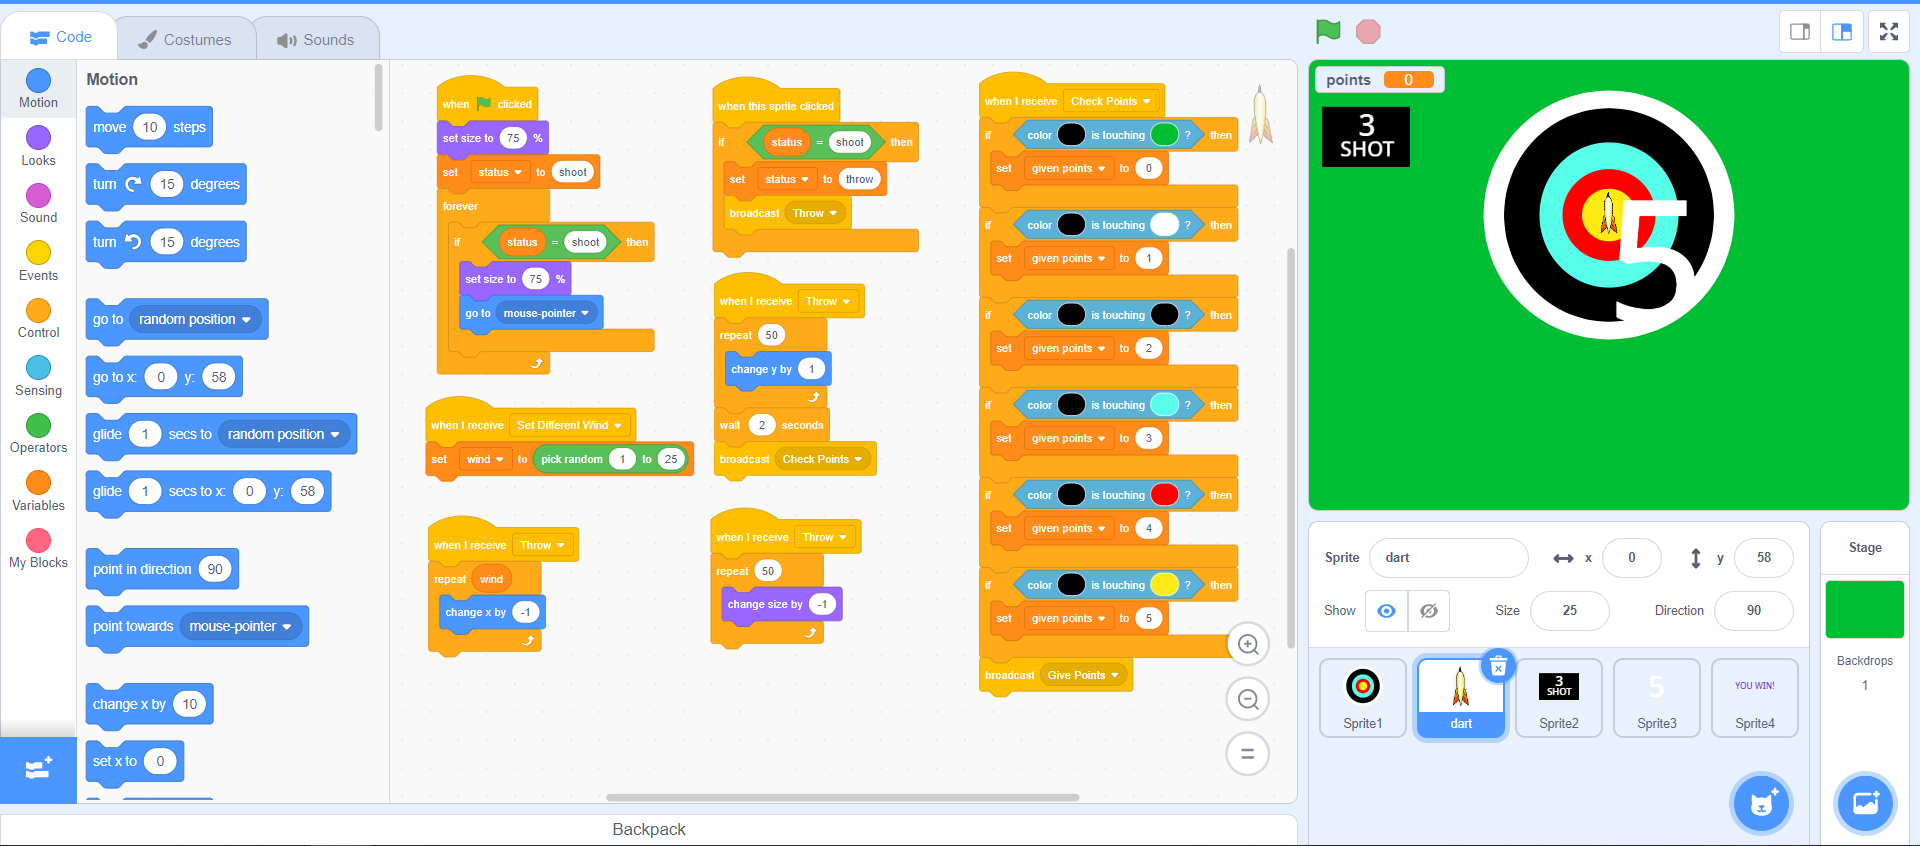
\includegraphics[width=1.0\linewidth,height=0.5\linewidth]{fig150013.png}
  \caption{Отклоняване на стрелата встрани}
\label{fig150013}
\end{figure}

\section{Програмиране на героя, който отброява броя изстрели}

В тази стъпка ще добавите инструкции, които ще показват на играча колко изстрела още има право да направи. За целта изберете героя, който добавихте за брой изстрели. Поставете този герой на избрана от вас позиция. Създайте нова променлива, която ще съдържа в себе си броя на изтрелите. След това направете нужните проверки - ако броя на изстрелите е 3, то тогава трябва да се премине към костюм, който показва три изстрела, ако броя на изстрелите е две - то тогава трябва да се премине към костюма с два изстрела и т.н. При последната проверка - ако броя на изстрелите е 0, то тогава трябва да се изпрати съобщение, че играта е приключила.

\begin{figure}[H]
  \centering
  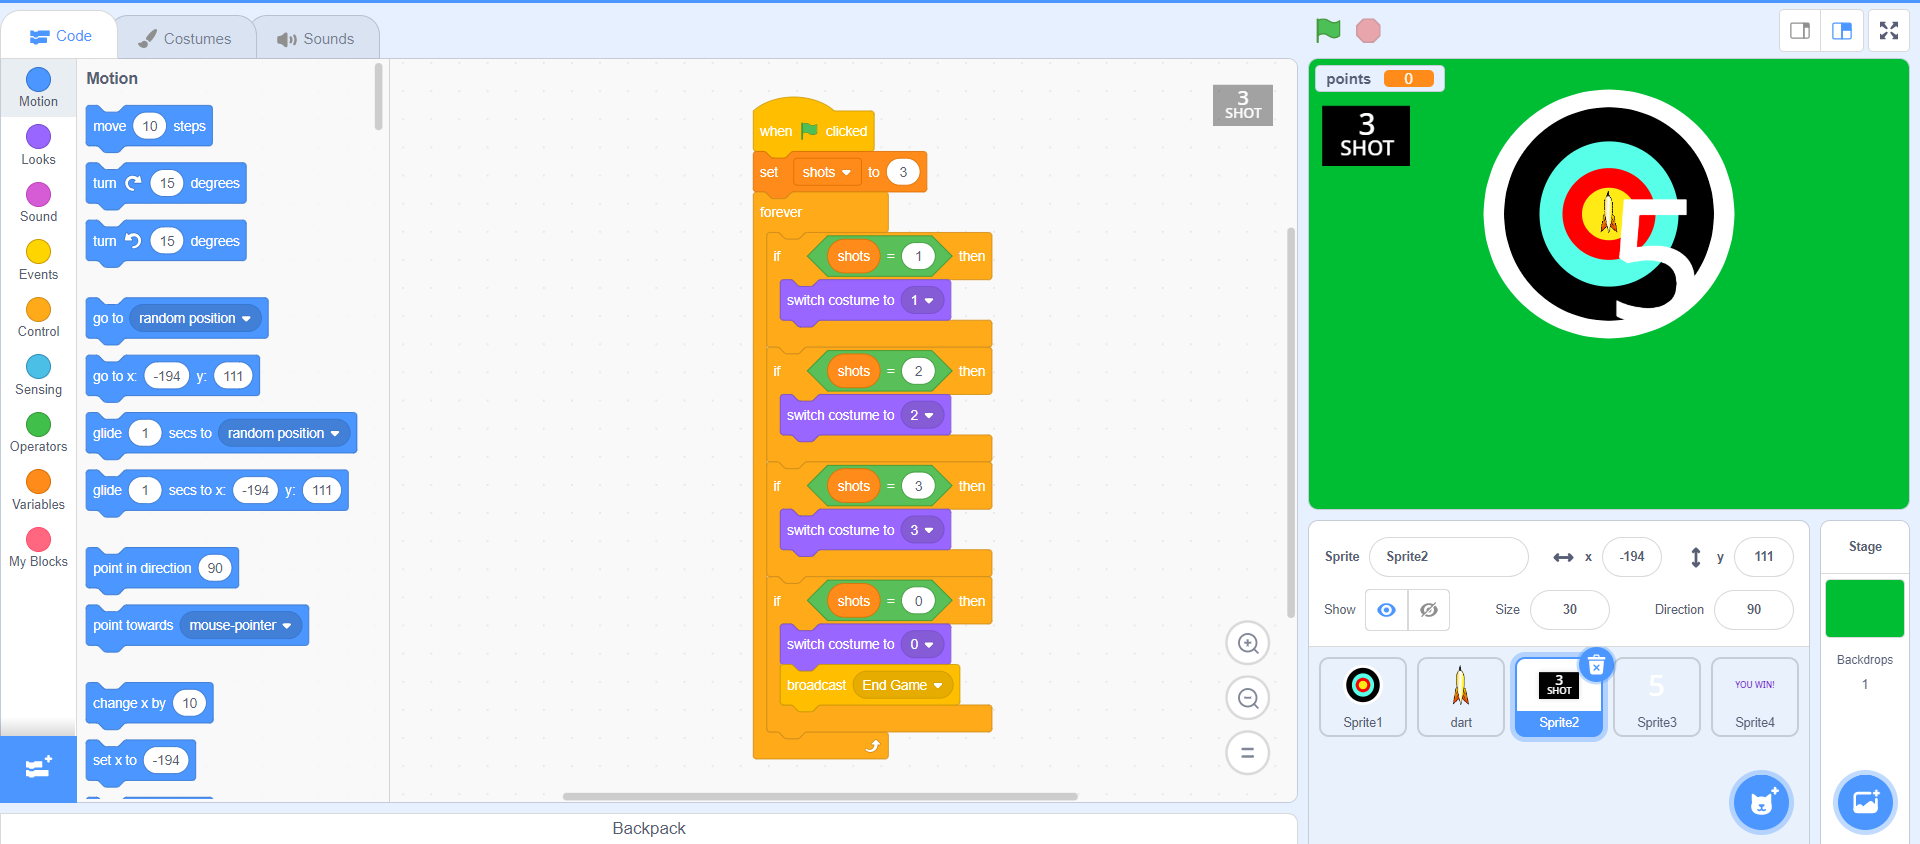
\includegraphics[width=1.0\linewidth,height=0.5\linewidth]{fig150014.png}
  \caption{Програмиране на брой изстрели}
\label{fig150014}
\end{figure}

\section{Програмиране на героя, който показва броя на точките}

Изберете героя, който показва колко точки е спечелил играчът. Този герой освен за това да покаже колко са точките, той ще отговаря и за това да намали броя на изстрелите, да зададе нова посока на вятъра, както и да промени статуса на стрелката да бъде готова отново за изстрел.

Тъй като не знаете колко точки ще спечели играчът и за да не правите хиляди проверки, може да си скръсисте имената на костюмите на броя точки. Така лесно ще може да преминавате от костюм на костюм, тй като имате променлива, която държи в себе си броя на текущо спечелените точки.

\begin{figure}[H]
  \centering
  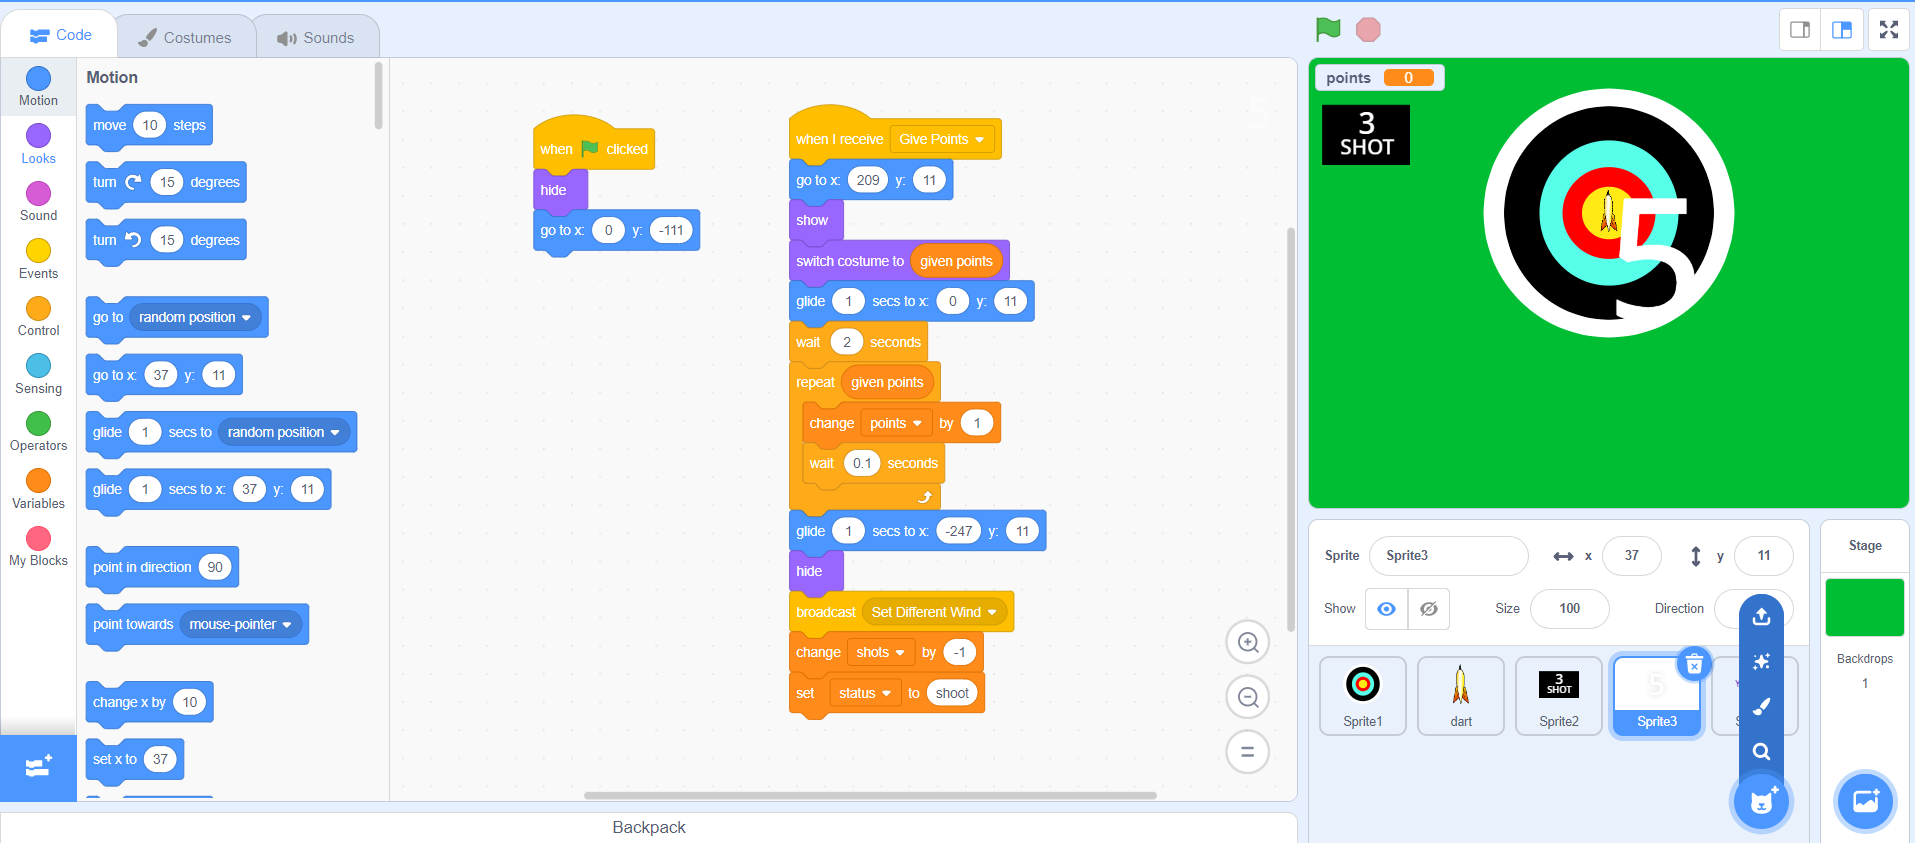
\includegraphics[width=1.0\linewidth,height=0.5\linewidth]{fig150015.png}
  \caption{Програмиране броя на точките}
\label{fig150015}
\end{figure}

\section{Програмиране края на играта}

Последната стъпка, която остана да направите е да програмирате края на играта. Спрямо това колко точки е спечелил играчът той или ще спечели или ще загуби след третия изстрел. Ако броя на точките е по- голям от 13 - той печели. В противен случай той губи.

\begin{figure}[H]
  \centering
  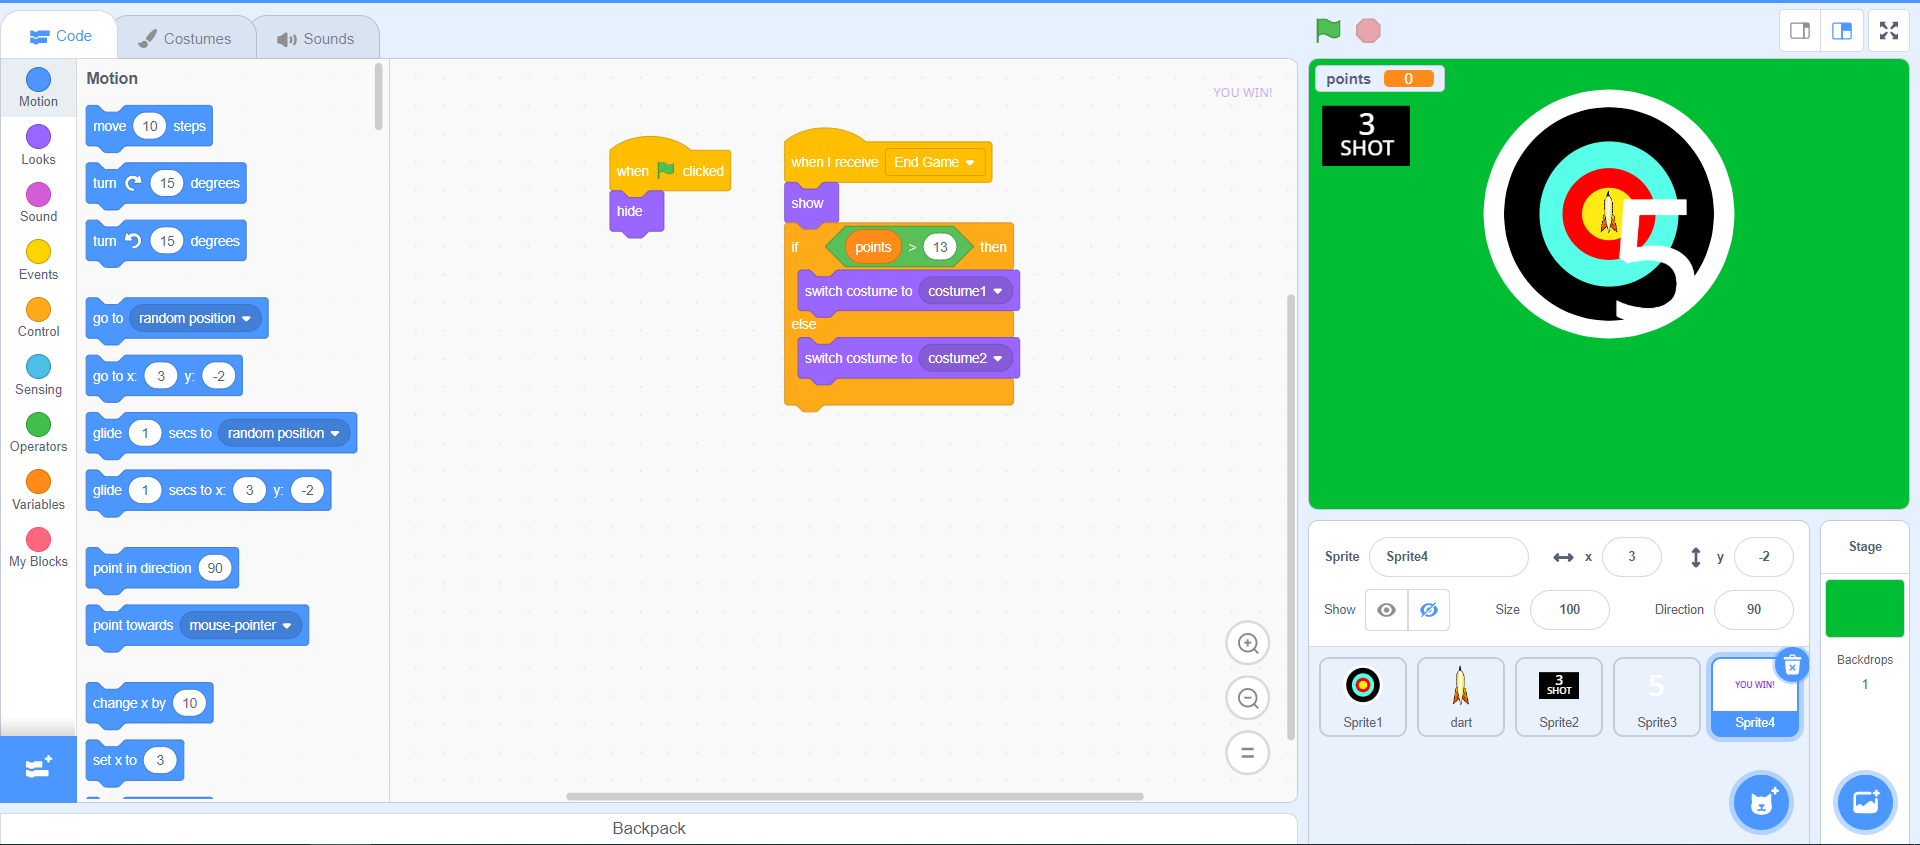
\includegraphics[width=1.0\linewidth,height=0.5\linewidth]{fig150016.png}
  \caption{Програмиране края на играта}
\label{fig150016}
\end{figure}

Готови сте да проверите колко сте точни и добри в играта, която създадохте.